\chapter{Positioning system : a two-threaded server}
 \section{Why use sockets and not JavaEE ?}
  \indent The server is linked with the other devices through TCP sockets. We use such a technology and not     JavaEE because sockets are more appropriate for our needs. Indeed, as our server is communicating with the TP-Link devices with a custom protocol through sockets, the same could be applied for the mobile device. JavaEE is a wonderful technology and has many advantages but it must go through the HTTP/S protocol through a specific port. Besides, a JavaEE server application needs a lot of configuration beforehand (or Spring annotations) whereas only one configuration file is required for sockets.\\
\indent Moreover, a socket-implemented server can be a standalone application, run as .jar file for example, unlike a JavaEE application, which first has to be packaged as a .war file\footnote{\textbf{war} : \textbf{W}eb \textbf{AR}chive, structured archive composed of a /META-INF and a /WEB-INF root directories containing all additional libraries and mandatory .class files.} file, then deployed on a ServletContainer (such as Tomcat, JBoss, etc\ldots). Proceeding as such makes tests and debug sessions much harder as it takes more time than to simply execute an application.\\

     \begin{figure}[H]
      \centering
      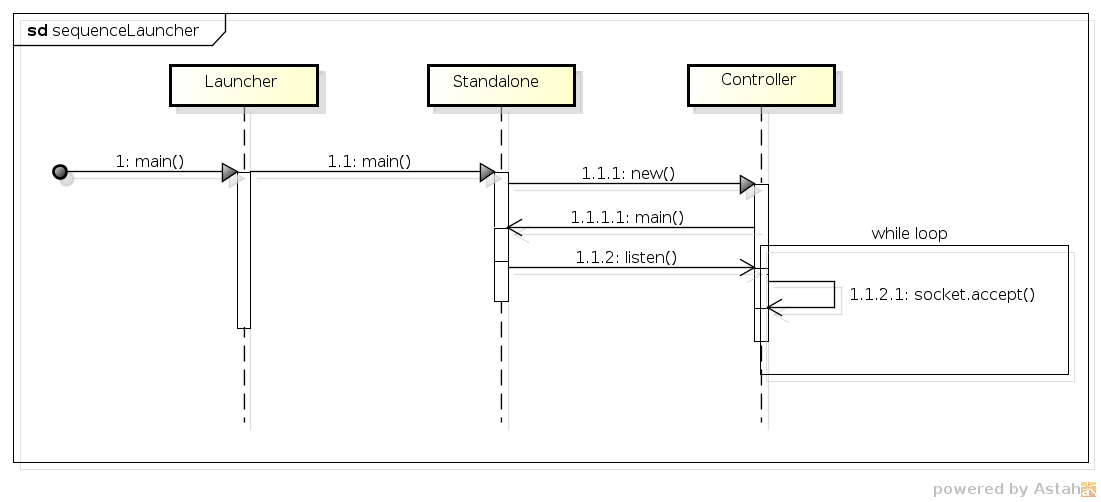
\includegraphics[scale = 0.5]{img/server/SequenceDiagramLauncher.png}
      \caption{Sequence Diagram representing the initialization of the server.}
      \label{fig:serv_init_seq_diagram}
     \end{figure}

  \subsection{Architecture of the server}
    Concerning the architecture, it is started through the Launcher.java class. It creates two threads that respectively instantiate two controllers : CalibrateController and LocateController. Our project respects the Service Oriented Architecture\footnote{Also known as SOA. Architecture model composed of layers. In our case, there are three layers : controller, service and repository.}. Each of these controllers possesses as attribute a ServerSocketChannel waiting for entering connections from mobile phones and each of these ServerSocketChannels are bound to a specific port. The first one is used to handle mobile devices calibration requests and the other one answers positioning requests.\\ 
\indent The controllers use SocketChannels (with a Selector) and which are non-blocking socket (unlike normal TCP). The principle is simple, one registers a ServerSocketChannel inside the Selector object and then waits for any entering connections. When a client binds itself with the server, it then registers a new SocketChannel inside the selector which can be accessed afterwards. However when one handles these channels, the order cannot be respected as the selector is just an encapsulated set. \\
\indent Each controller can access the database through the service layer with the classes CalibrateService and LocateService. Finally, these services are linked with the repository layer which has access to the database. 

     \begin{figure}[H]
      \centering
      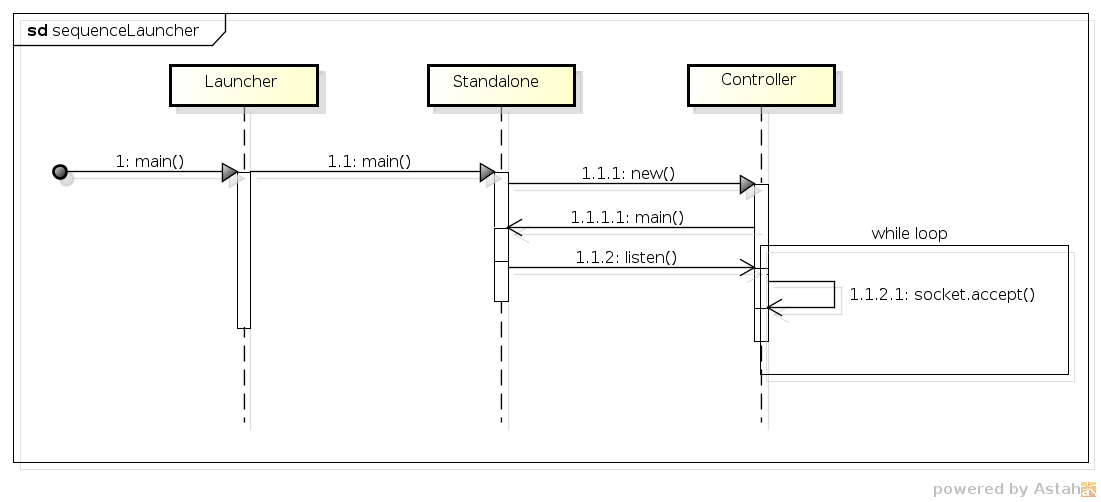
\includegraphics[scale = 0.5]{img/server/SequenceDiagramLauncher.png}
      \caption{Class Diagram showing the architecture of the server.}
      \label{fig:serv_class_diagram}
     \end{figure}

  \subsection{Socket Channels replacing Threads}
   \subsubsection{Advantage of Socket Channels}
    We first used normal TCP ServerSocket Java objects but the number of thread created was too important. It used to start as many threads as mobile devices' requests and for each request, for all APs, a new thread was started in addition to ask associated RSSI values. The performance was too dependent from the hosting computer's number of processors. This is why we changed the architecture thanks to the Java "\textit{Selector}" object.       
    
    \subsubsection{Handling of channels}
\indent Our implementation divides three types of channels :
    \begin{itemize}
     \item[$\rightarrow$] connectable channels;
     \item[$\rightarrow$] readable channels;
     \item[$\rightarrow$] writable channels.
    \end{itemize}
    \paragraph{Connectable Channels} They correspond to sockets which tried to bind themselves with the server. Such channels are immediately registered in the Selector as 'READABLE'.
    \paragraph{Readable Channels} They are the most important ones. When handling some, the data sent by the mobile device is parsed. It communicates then with the APs to have the associated RSSIs. Eventually, the database is accessed in order to query or insert values.
    \paragraph{Writable Channels} This channel is used to send back a response to the mobile device. When it is done writing, it finally closes the client's SocketChannel.

    \begin{figure}[H]
      \centering
      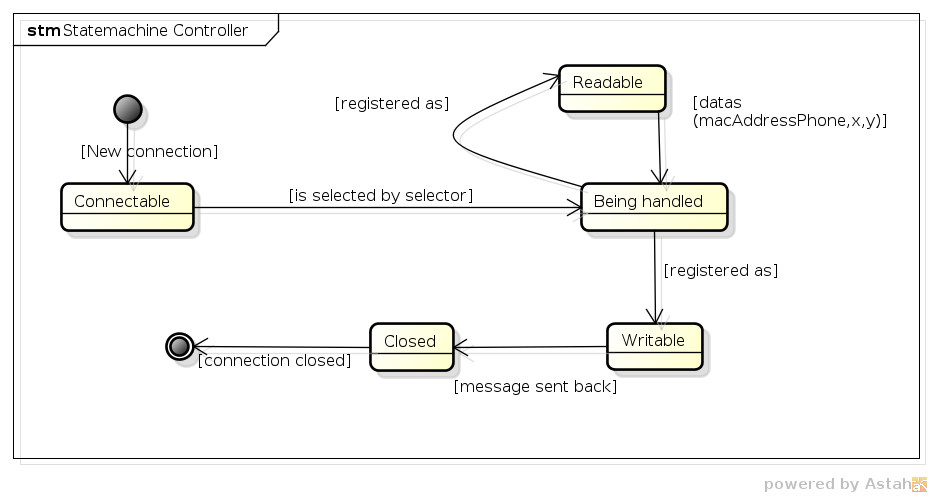
\includegraphics[scale = 0.40]{img/server/StatemachineDiagramController.png}
      \caption{State machine representing the handling of channels.}
      \label{fig:controller_statemachine}
    \end{figure}
    
   
  \subsection{Service Oriented Architecture}
   The SOA is an architecture whose purpose is to completely divide jobs to perform by the means of different layers. In this project, three layers have been created : the controller one, the service one and the repository one. Each one of them have a different role. The advantage of this architecture is that if someday, the way to access the database has changed for example, one will not have to modify the whole code but just the repository layer by adding a new DAO\footnote{\textbf{DAO} : \textbf{D}ata \textbf{A}ccess \textbf{O}bject. Interface providing a way of converting database objects into standard Java Objects.} class.
   
   \paragraph{Controller layer} It is where the endpoints of the server are stored. The role they have to carry out is to : listen to any entering connection from a client, control the consistency of the request, perform some mandatory tasks and finally relay the information to the service layer.
   
   \paragraph{Service layer} Intermediary layer linked to the controller and the repository layer. Its existence allows not to let the controllers have a direct access to the repository and access directly the database.
   
   \paragraph{Repository layer} Model-linked layer. It accesses the data which can be stored in different way (database, files, etc\ldots) and can perform CRUD\footnote{\textbf{CRUD} : \textbf{C}reate, \textbf{R}ead, \textbf{U}pdate, \textbf{D}elete, operations which can be performed on a database.} operations.
  
  \begin{center}
     These are the class diagrams of the communication between the different devices: %TODO pluriel/singulier
     \begin{figure}[H]
      \centering
      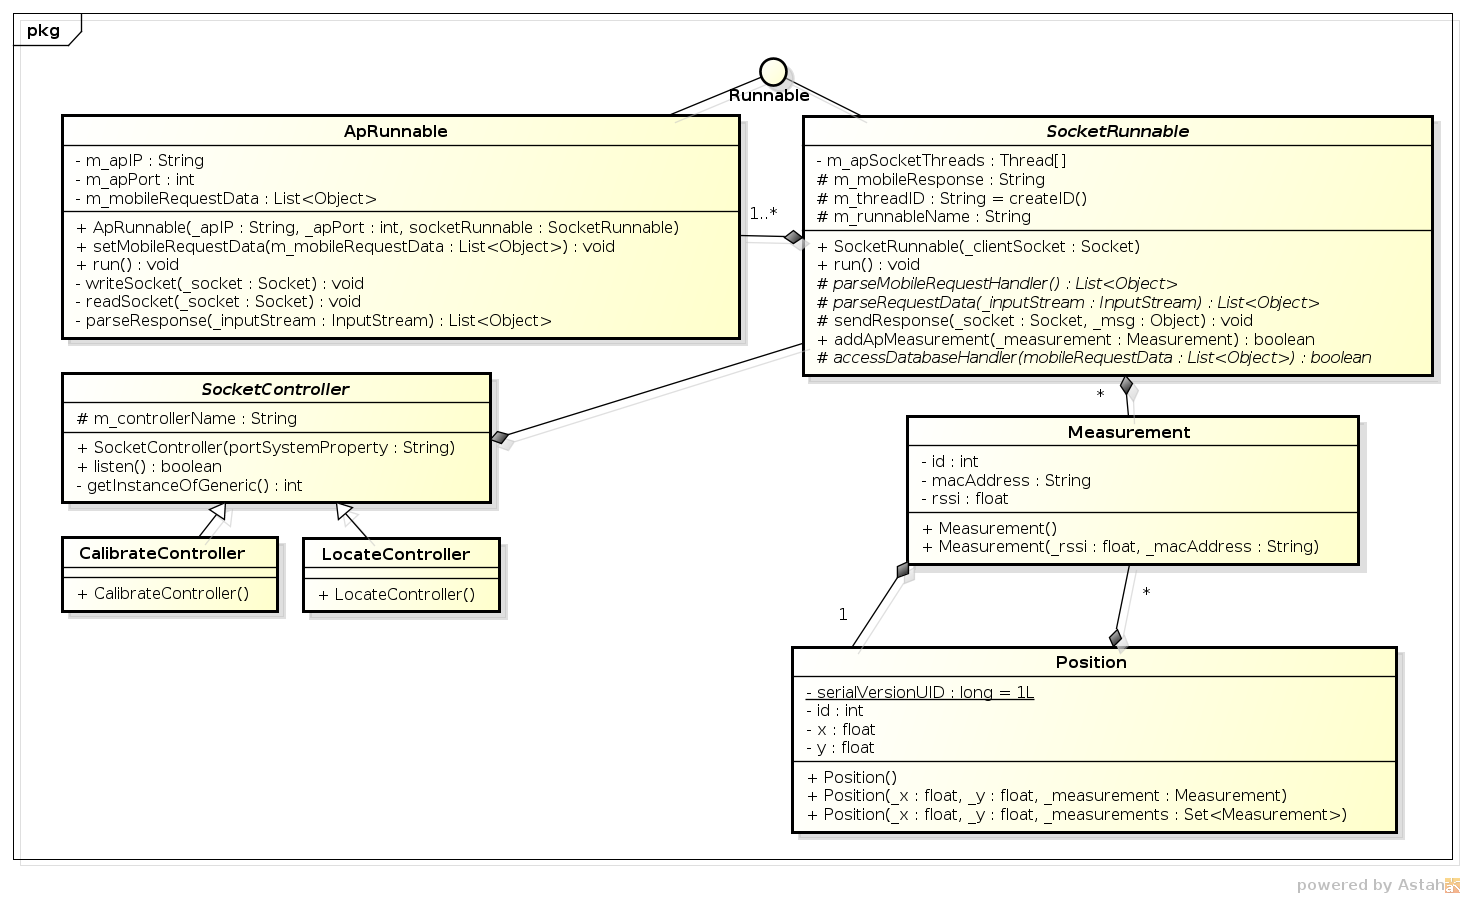
\includegraphics[scale = 0.40]{img/server/classDiagramController.png}
      \caption{Class diagram showing the classes communicating with the controllers.}
      \label{fig:controller_class_diagram}
     \end{figure}

     \begin{figure}[H]
      \centering
      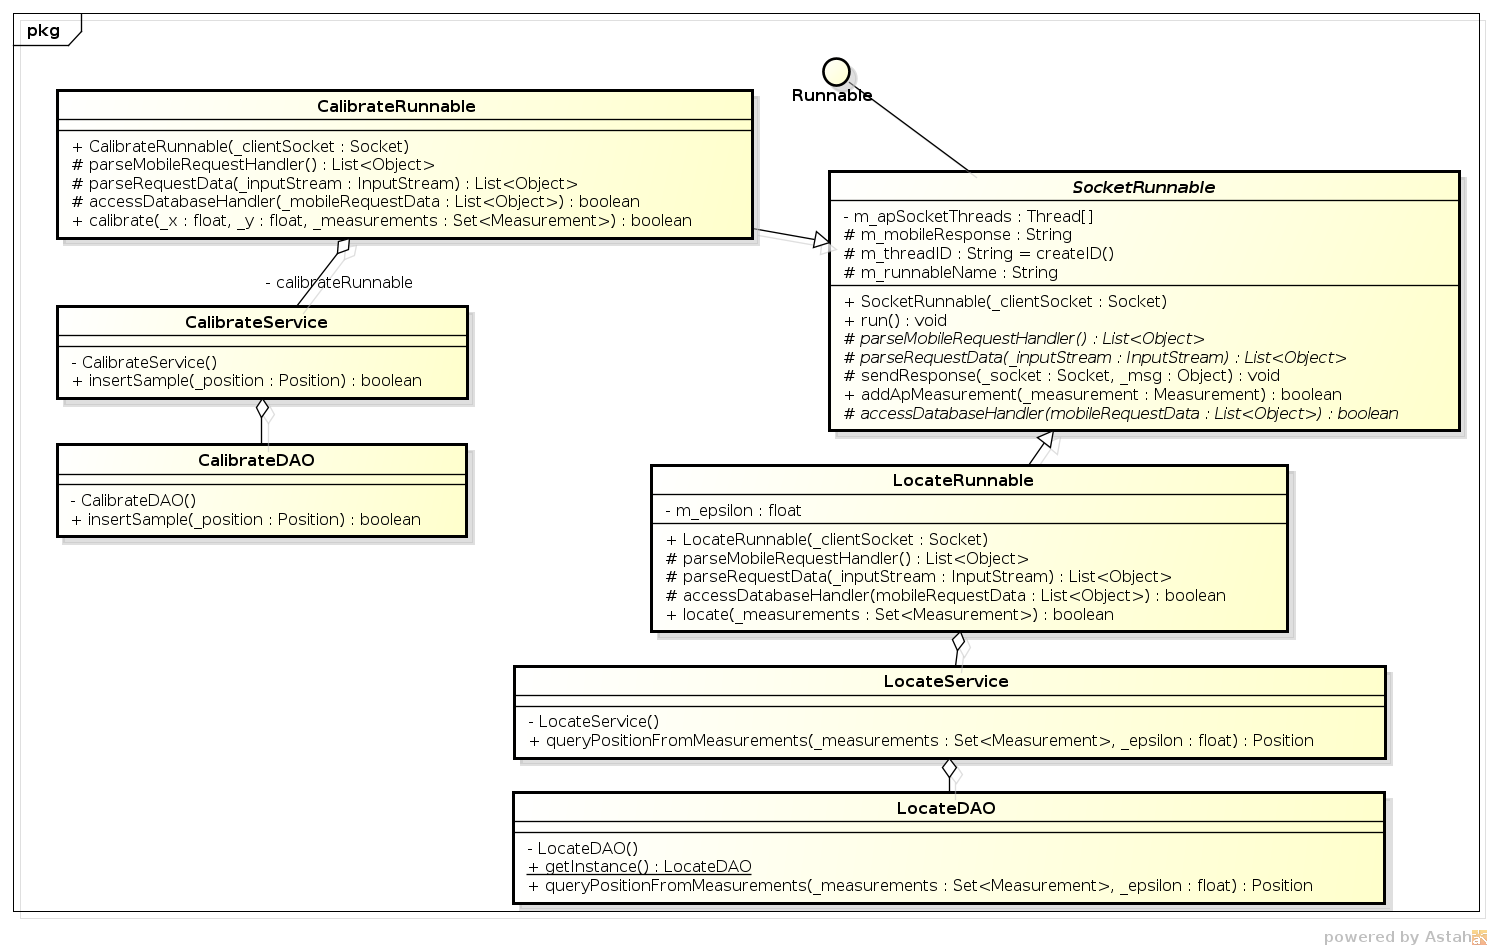
\includegraphics[scale = 0.40]{img/server/classDiagramDAO.png}
      \caption{Class diagram representing the way the database is accessed from controllers.}
      \label{fig:dao_class_diagram}
     \end{figure}
   \end{center}     
    
  \subsection{A database accessed through ORM}
   \subsubsection{Database side}
  The project's database is in PostgreSQL language because it has several interesting advantages. For instance, it is known to never crash, it is quite practical unlike other language concerning tables management and moreover, it is an open source software. \\
\indent The database contains two main tables, "Position" and "Measurement", linked to each other with a one-to-many$\leftrightarrow$many-to-one relationship :

     \begin{figure}[H]
      \centering
      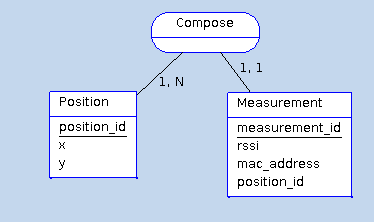
\includegraphics[scale = 0.7]{img/server/Database_MCD_Merise.png}
      \caption{Merise MCD showing the database's table relationships.}
      \label{fig:db_mcd_diagram}
     \end{figure}

  \subsubsection{Server side}
  Nowadays, there are two main ways to obtain server side (in Java), data from a database : JDBC and Hibernate.
    \paragraph{Java DataBase Connectivity} It consists in accessing directly the database by creating an instance of connection. CRUD operations can then be executed as statements and eventually the connection has to be closed at the end of the access. This way of interacting with the database is not very efficient when one needs to perform many connections as one has to open and close connections each time.
    \paragraph{Hibernate} API used for database object persistence in Java (or ORM\footnote{\textbf{ORM} : \textbf{O}bject \textbf{R}elationnal \textbf{M}apping}.). It can convert by the means of configuration files, database objects into POJO\footnote{\textbf{POJO} : \textbf{P}lain \textbf{O}ld \textbf{J}ava \textbf{O}bject, standard Java objects (in contrary of Java Beans for example).}s. It is also able to reproduce relationships and linked tables. It works thanks to the "session" concept. Each time one has to access the database, one asks to get a new instance of Hibernate session where one will be able to perform CRUD operations more easily than JDBC. Some methods are already implemented in order to facilitate such operations. This is the technology used in this project. Three configuration files were required : 
    \begin{itemize}
    \item[$\rightarrow$] \textit{hibernate.cfg.xml}, which defines how Hibernate can access the database and which tables have to be linked to which Java class (in our case, Position.java and Measurement.java);
    \item[$\rightarrow$] \textit{Position.hbm.xml}, which corresponds to how can the database table "Position" can be mapped to this Java class;
    \item[$\rightarrow$] \textit{Measurement.hbm.xml}, which corresponds to how can the database table "Measurement" can be mapped to this Java class;
    \end{itemize}
  
  \subsection{How communication is performed between devices ?}
    An overall sequence diagram has been created in order to look how a mobile request is handled all the way to the end.
    
    
 \begin{sidewaysfigure}
     \rotatebox{0}{
       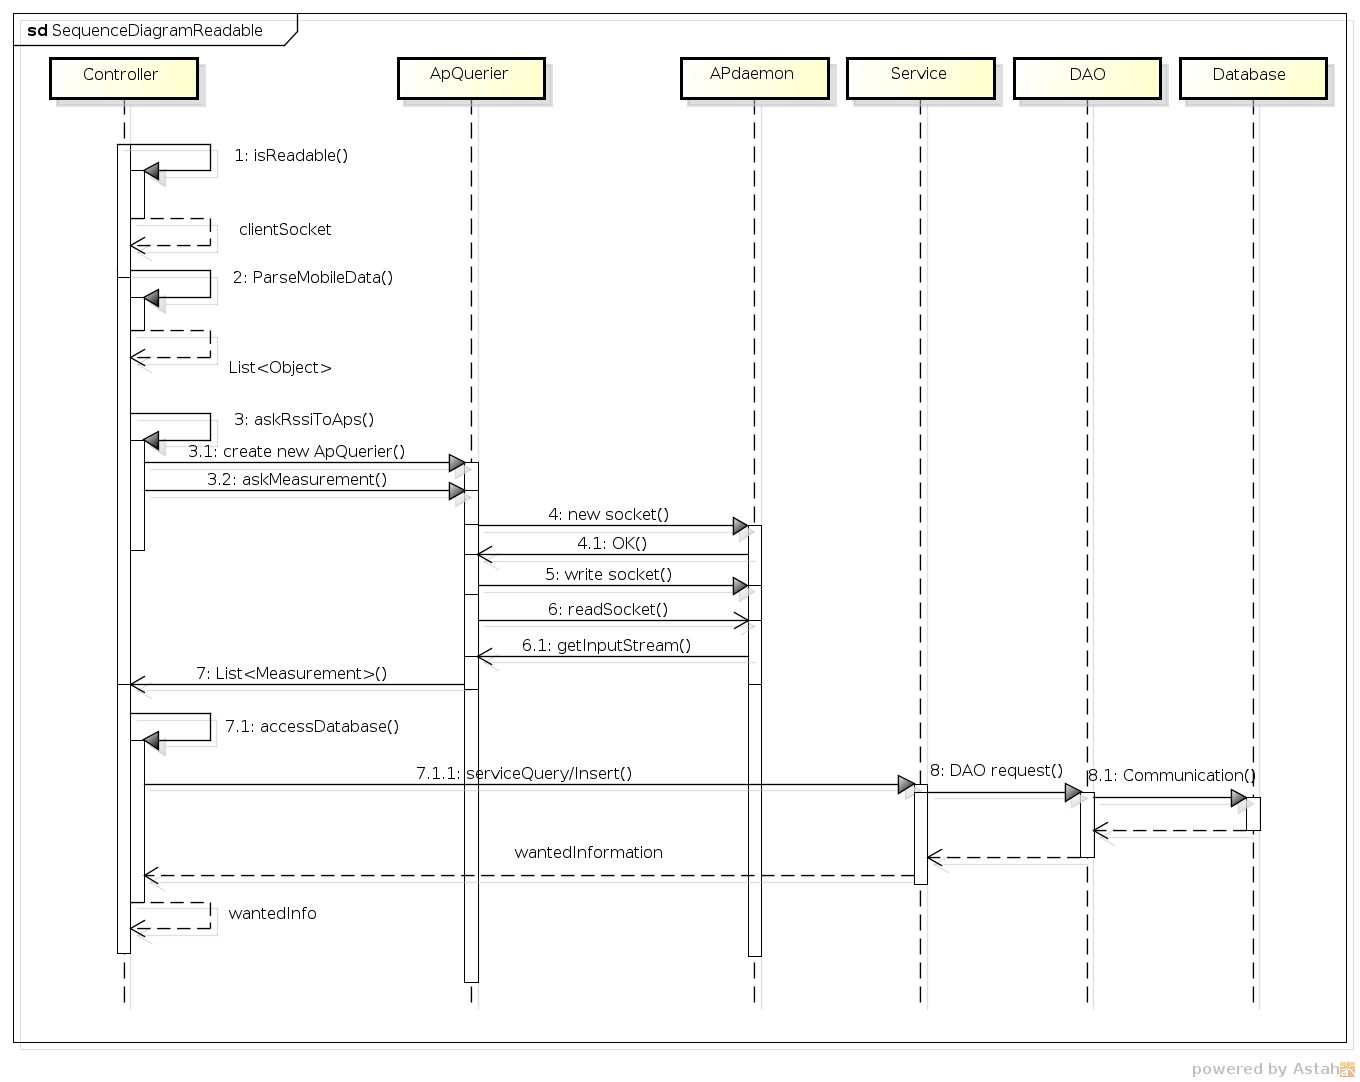
\includegraphics[scale = 0.55]{img/server/SequenceDiagramReadable.png}
      }
      \caption{Sequence diagram of the handling of a readable socket.}
      \label{fig:readable_seq_diag}
     \end{sidewaysfigure}
    \newpage
   ~\\
  \subsection{How are the errors managed ?}
    The server is running until the application is shut down by the server's administrator. So it must absolutely not crash. Hence when errors occurr, they are all cought and handled in a way allowing the server to continue running. In order to create such a error-proof architecture, one must be aware of all the states of the server, one must know the values of the different attributes when passed from methods to methods and the values of the returned objects.